\documentclass[12pt,letterpaper]{article}
\usepackage{color}
\usepackage{graphicx}
\usepackage{geometry}
\usepackage{setspace}
\usepackage{anyfontsize}
\usepackage{parskip}
\usepackage{indentfirst}
\usepackage{amsmath}
\usepackage{natbib}
\usepackage{float}
\usepackage{subcaption}

\geometry{letterpaper, portrait, margin=1in}
\doublespace
\title{On Tessellation and Euclidean Patterns of Polygons}
\author{Tynan Purdy}
\date{\vspace{-5ex}}
\graphicspath{{../images/}}

\begin{document}
\large
\parindent=0.5in
{\fontsize{12}{14.4}
	{\singlespace
	\pagenumbering{gobble}
	\maketitle
	\begin{center}
	\vspace{4mm}
	002129-0004 \\
	\vspace{4mm}
	Math HL IA \\
	\vspace{4mm}
	May 2019 \\
	\vspace{4mm}
	Words: 352\\
	\end{center}
	}
}	

\newpage
\pagenumbering{arabic}
\begin{abstract}
Tessellation is the bridge between art and mathematics. It is the uniform patterning of a shape over a plane with no gaps between individual instances of the shape. Tessellations have existed in art and in architecture for thousands of years, dating back to early Islam. \citep{arabic} I am personally interested in tessellated patterns because they are relevant and applicable to graphic design and mechanical engineering. I use tessellations in Computer-Aided Design software for mechanical design and Adobe Illustrator for graphic and art projects. Both programs have functions for generating tessellations, and the methods behind those functions will be explored.
\end{abstract}

\newpage
\tableofcontents

\newpage
\section{Introduction}
Tessellation is everywhere. In a carpentered, geometric world, patterns of polygons make up almost everything around us, from ceiling tiles to brick sidewalks. Since tessellation is such a prominent occurrence, it should be understood what tessellation is, where it came from and how it is performed mathematically. 
\subsection{Historic Origins}
\subsubsection{Islamic Art}

\begin{figure}[H]
    \begin{center}
        \caption{Examples of Islamic tessellations \citep{arabic}}
        \label{fig:islam}
        \begin{subfigure}[b]{.3\linewidth}
            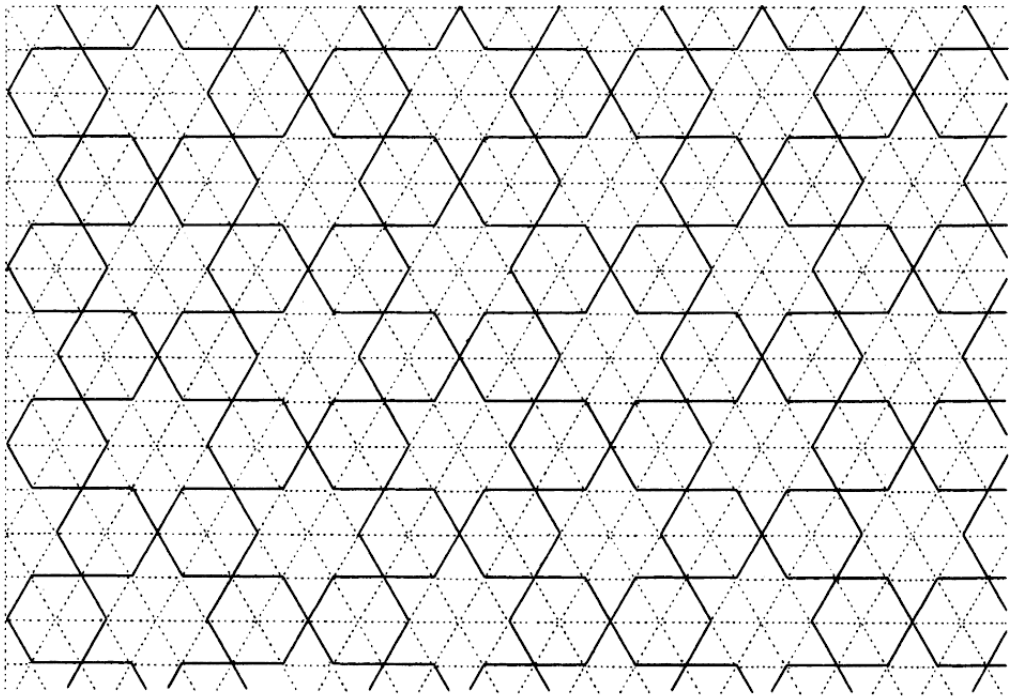
\includegraphics[width=\linewidth]{islam1}
        \end{subfigure}
        \begin{subfigure}[b]{.3\linewidth}
            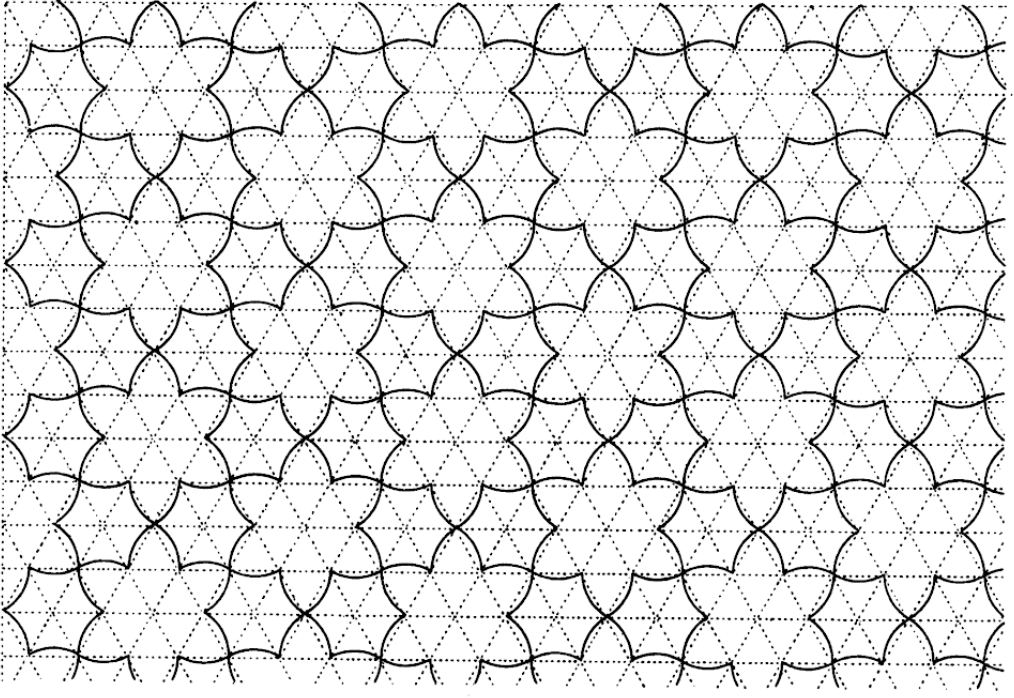
\includegraphics[width=\linewidth]{islam2}
        \end{subfigure}
        \begin{subfigure}[b]{.3\linewidth}
            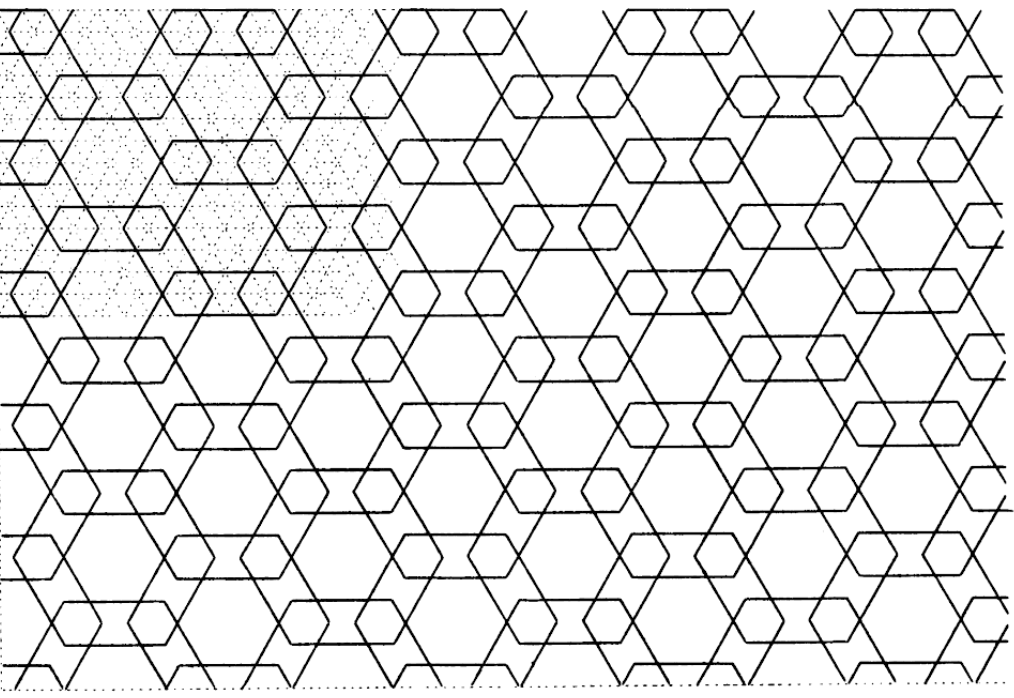
\includegraphics[width=\linewidth]{islam3}
        \end{subfigure}
    \end{center}
\end{figure}
\subsubsection{Nature}
Like many mathematical subjects, tessellation has manifestations in nature. The most popular natural example is beehive honeycombs.
\section{Tessellation}
Tessellations are described using the notation of the Schl\"afli symbol (\ref{eq:schlafli}), where $p$ is the number of edges and $q$ is the number of edges intersecting at a vertex.

\begin{equation}
    \label{eq:schlafli}
    \{p,q\}
\end{equation}

There are 3 regular tessellations using a single convex polygon with no gaps: rectangular grids, honeycombs, and triangular grids. These are by far the most commonly found tessellations.

\begin{figure}[H]
    \begin{center}
        \caption{Tessellation of rectangle $\{4,4\}$}
        \label{fig:square}
        \begin{subfigure}[b]{.3\linewidth}
            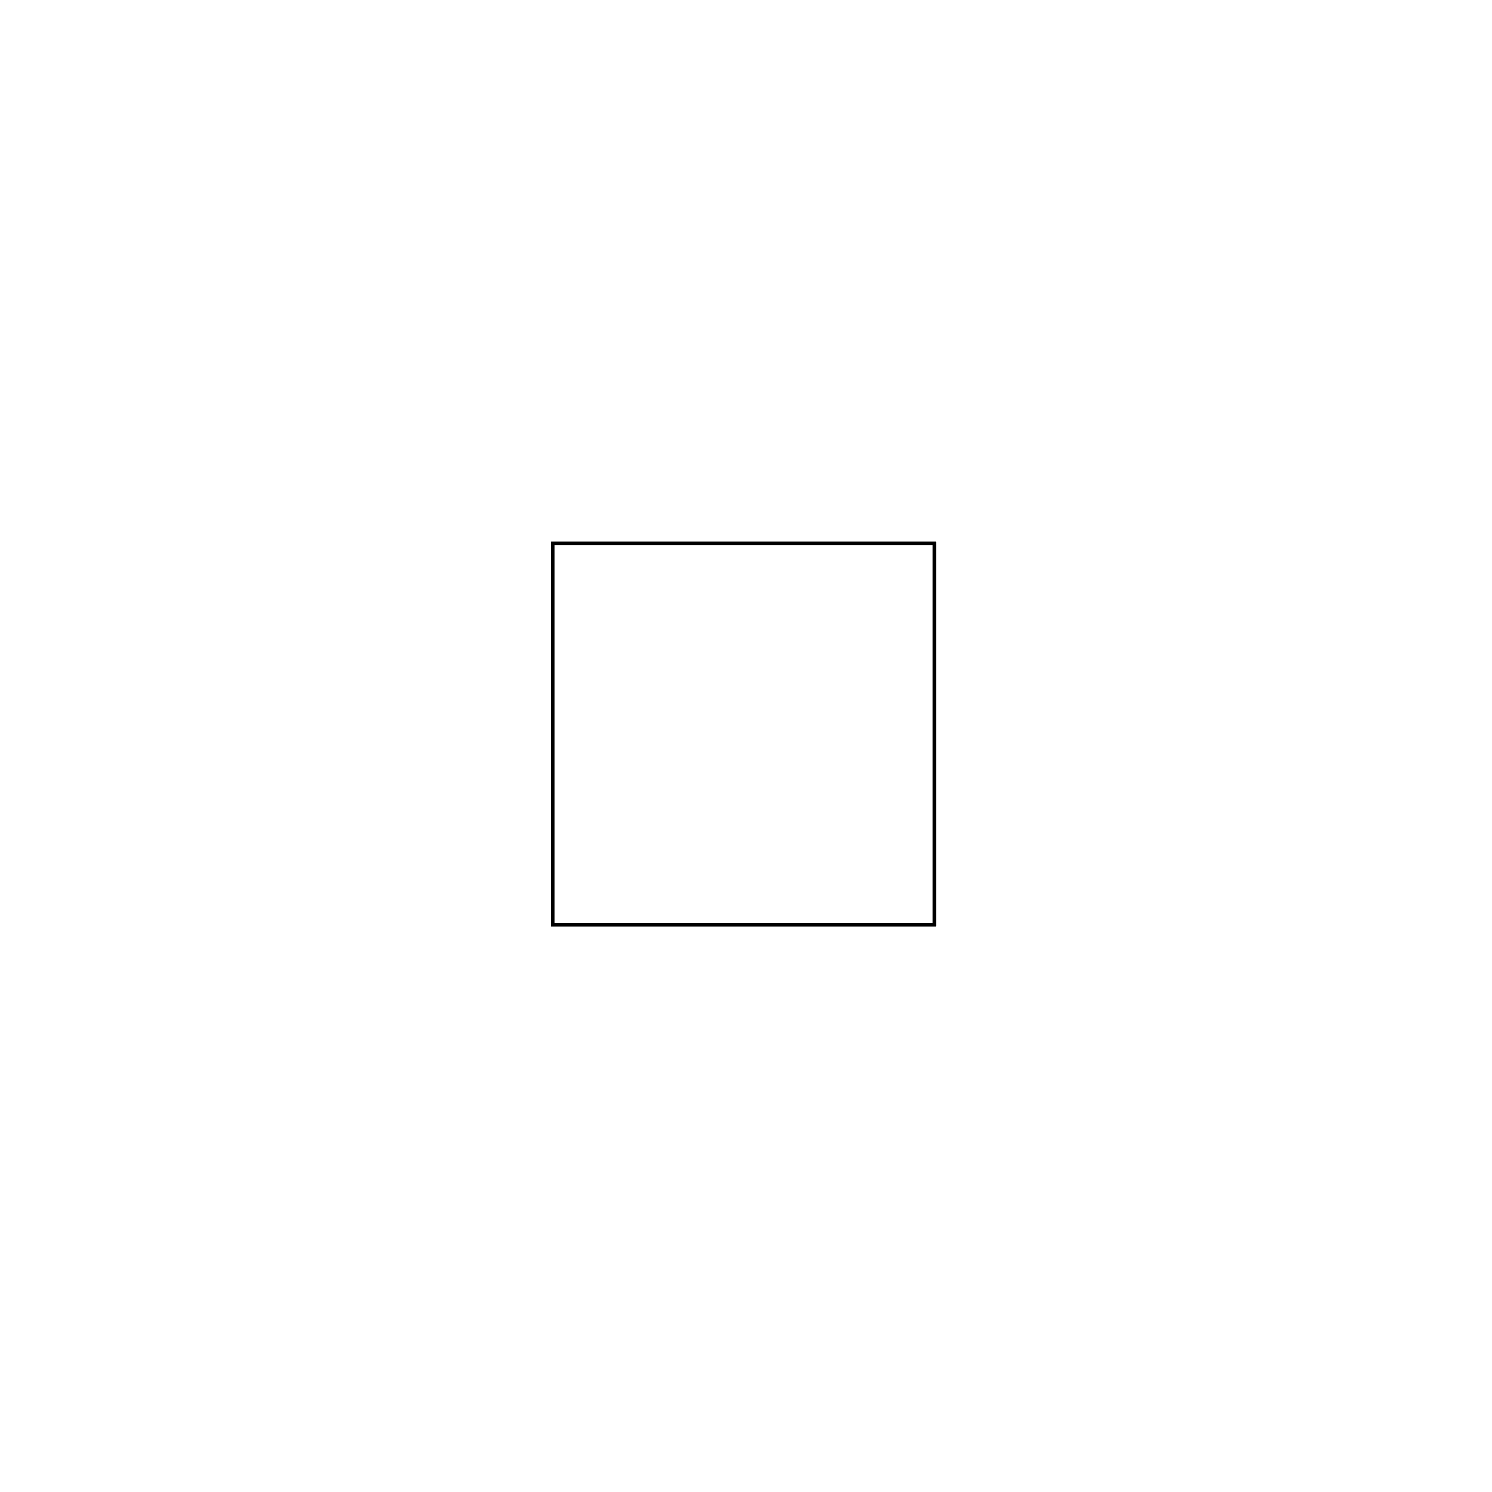
\includegraphics[width=\linewidth]{base-square}
            \caption{Base 4-sided shape}
        \end{subfigure}
        \begin{subfigure}[b]{.3\linewidth}
            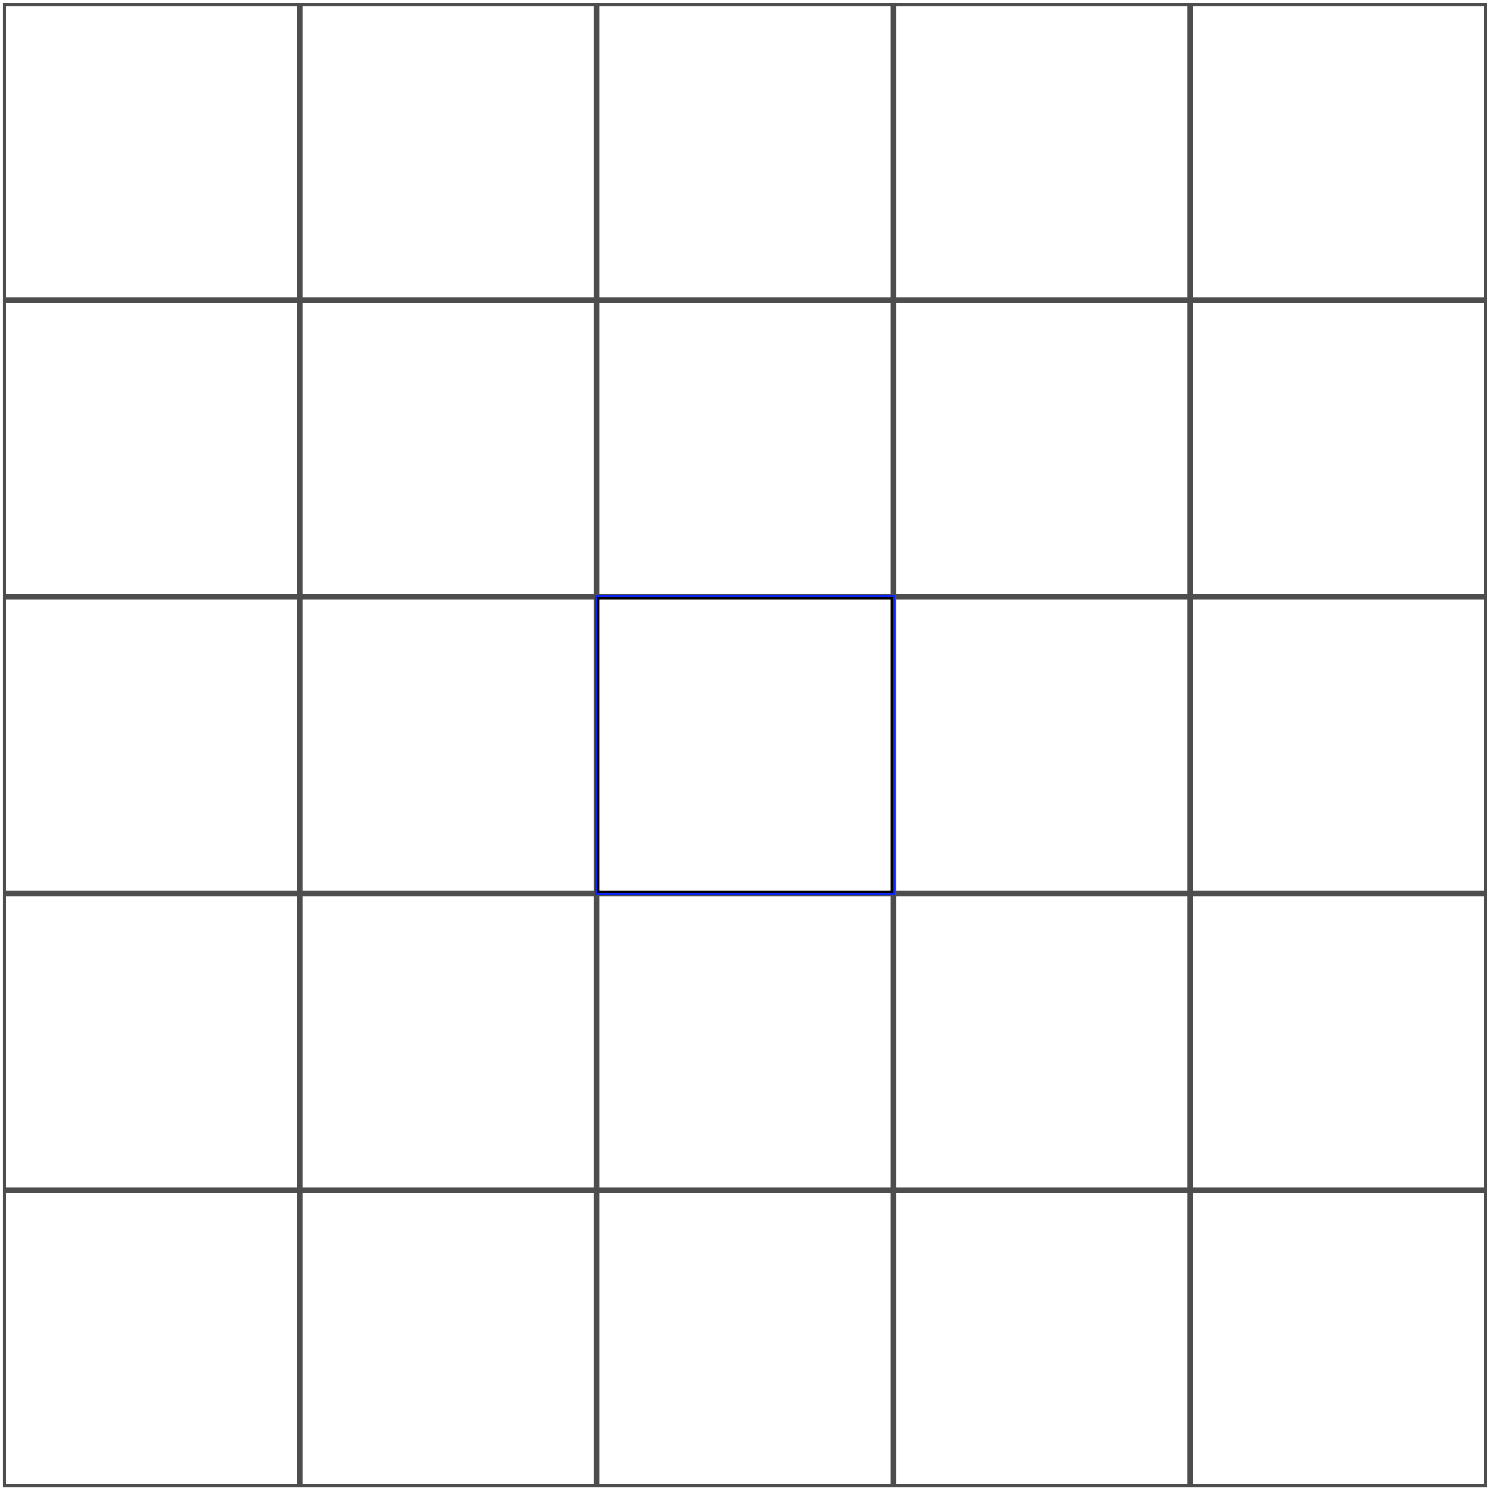
\includegraphics[width=\linewidth]{tes-square}
            \caption{5x5 tessellation}
        \end{subfigure}
    \end{center}
\end{figure}

\begin{figure}[H]
    \begin{center}
        \caption{Tesselation of a hexagon, also known as a honeycomb $\{6,3\}$}
        \label{fig:hex}
        \begin{subfigure}[b]{.3\linewidth}
            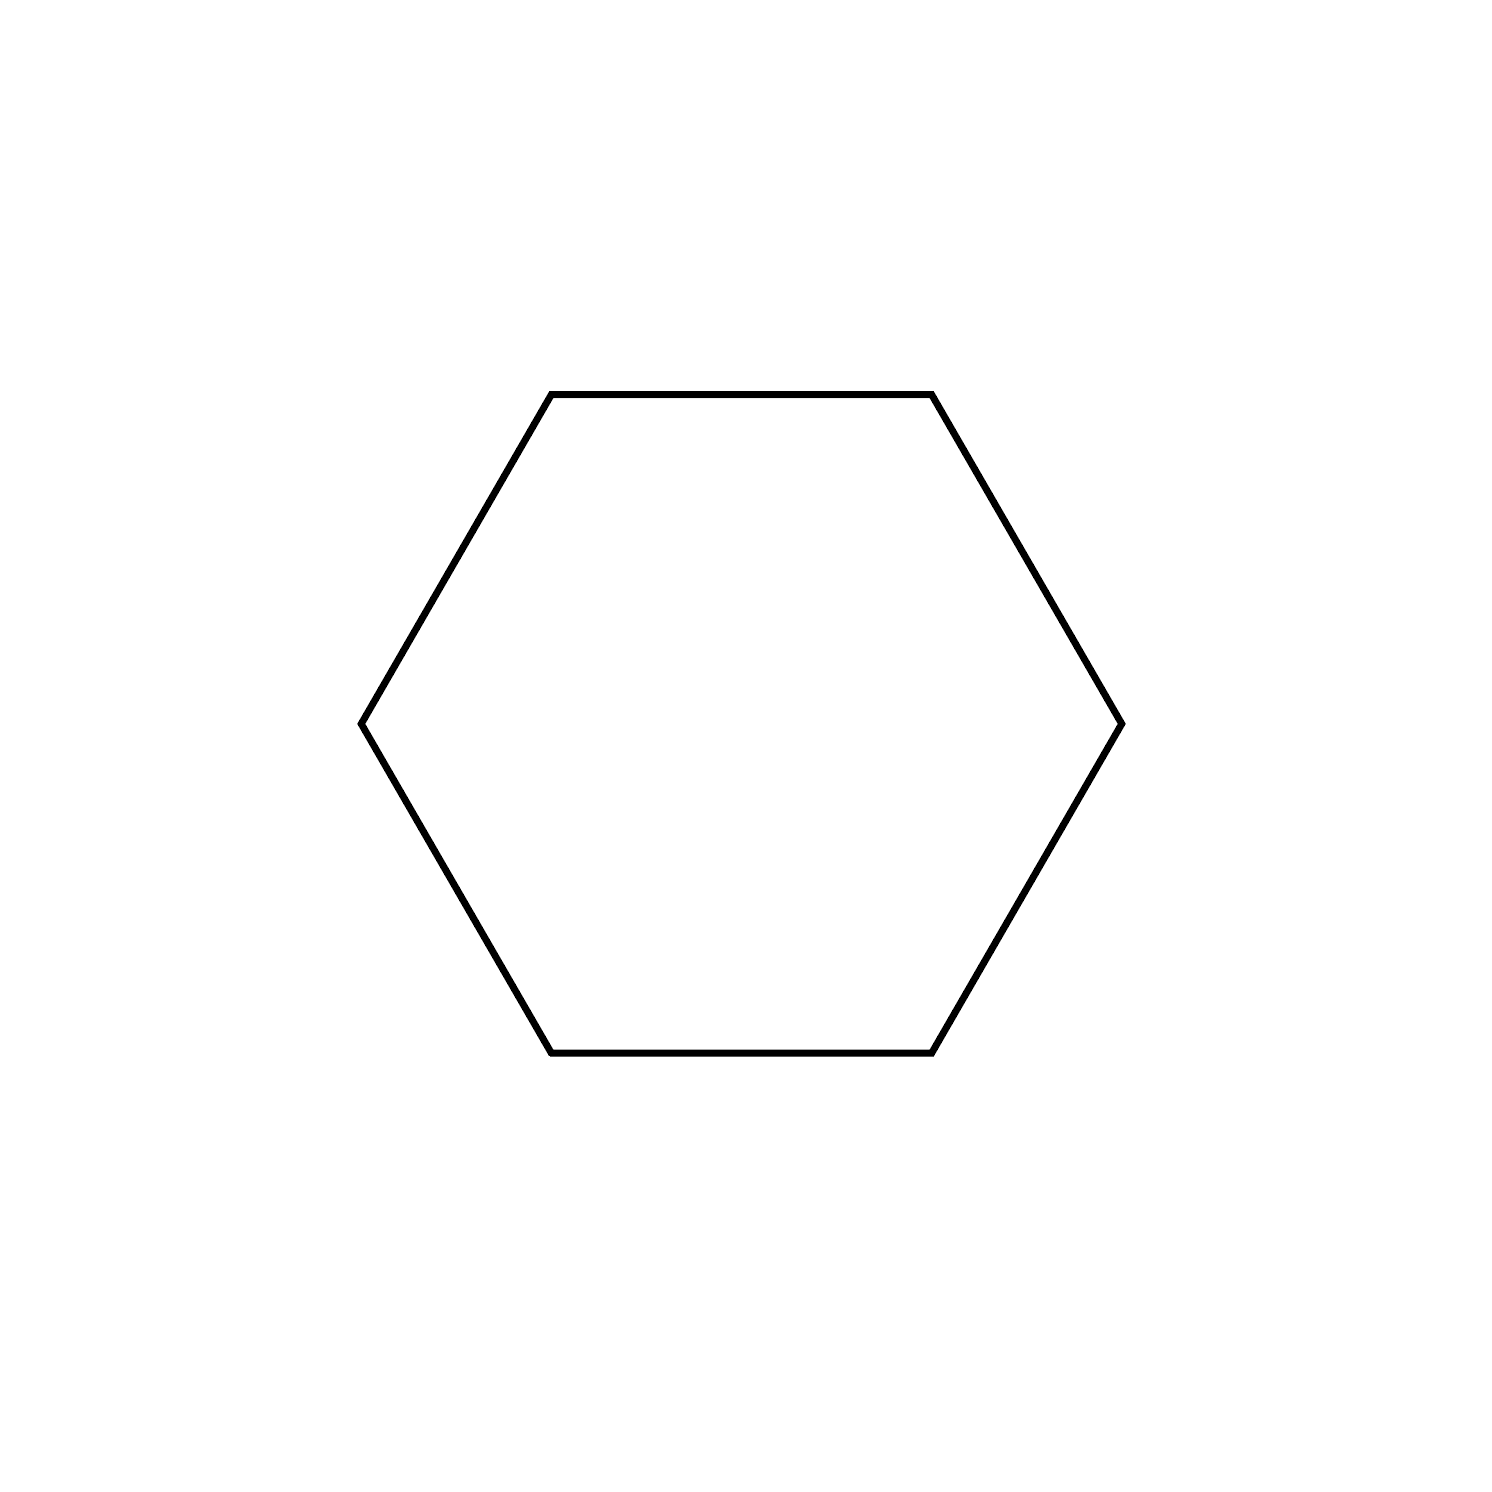
\includegraphics[width=\linewidth]{base-hex}
            \caption{Base 6-sided shape}
        \end{subfigure}
        \begin{subfigure}[b]{.3\linewidth}
            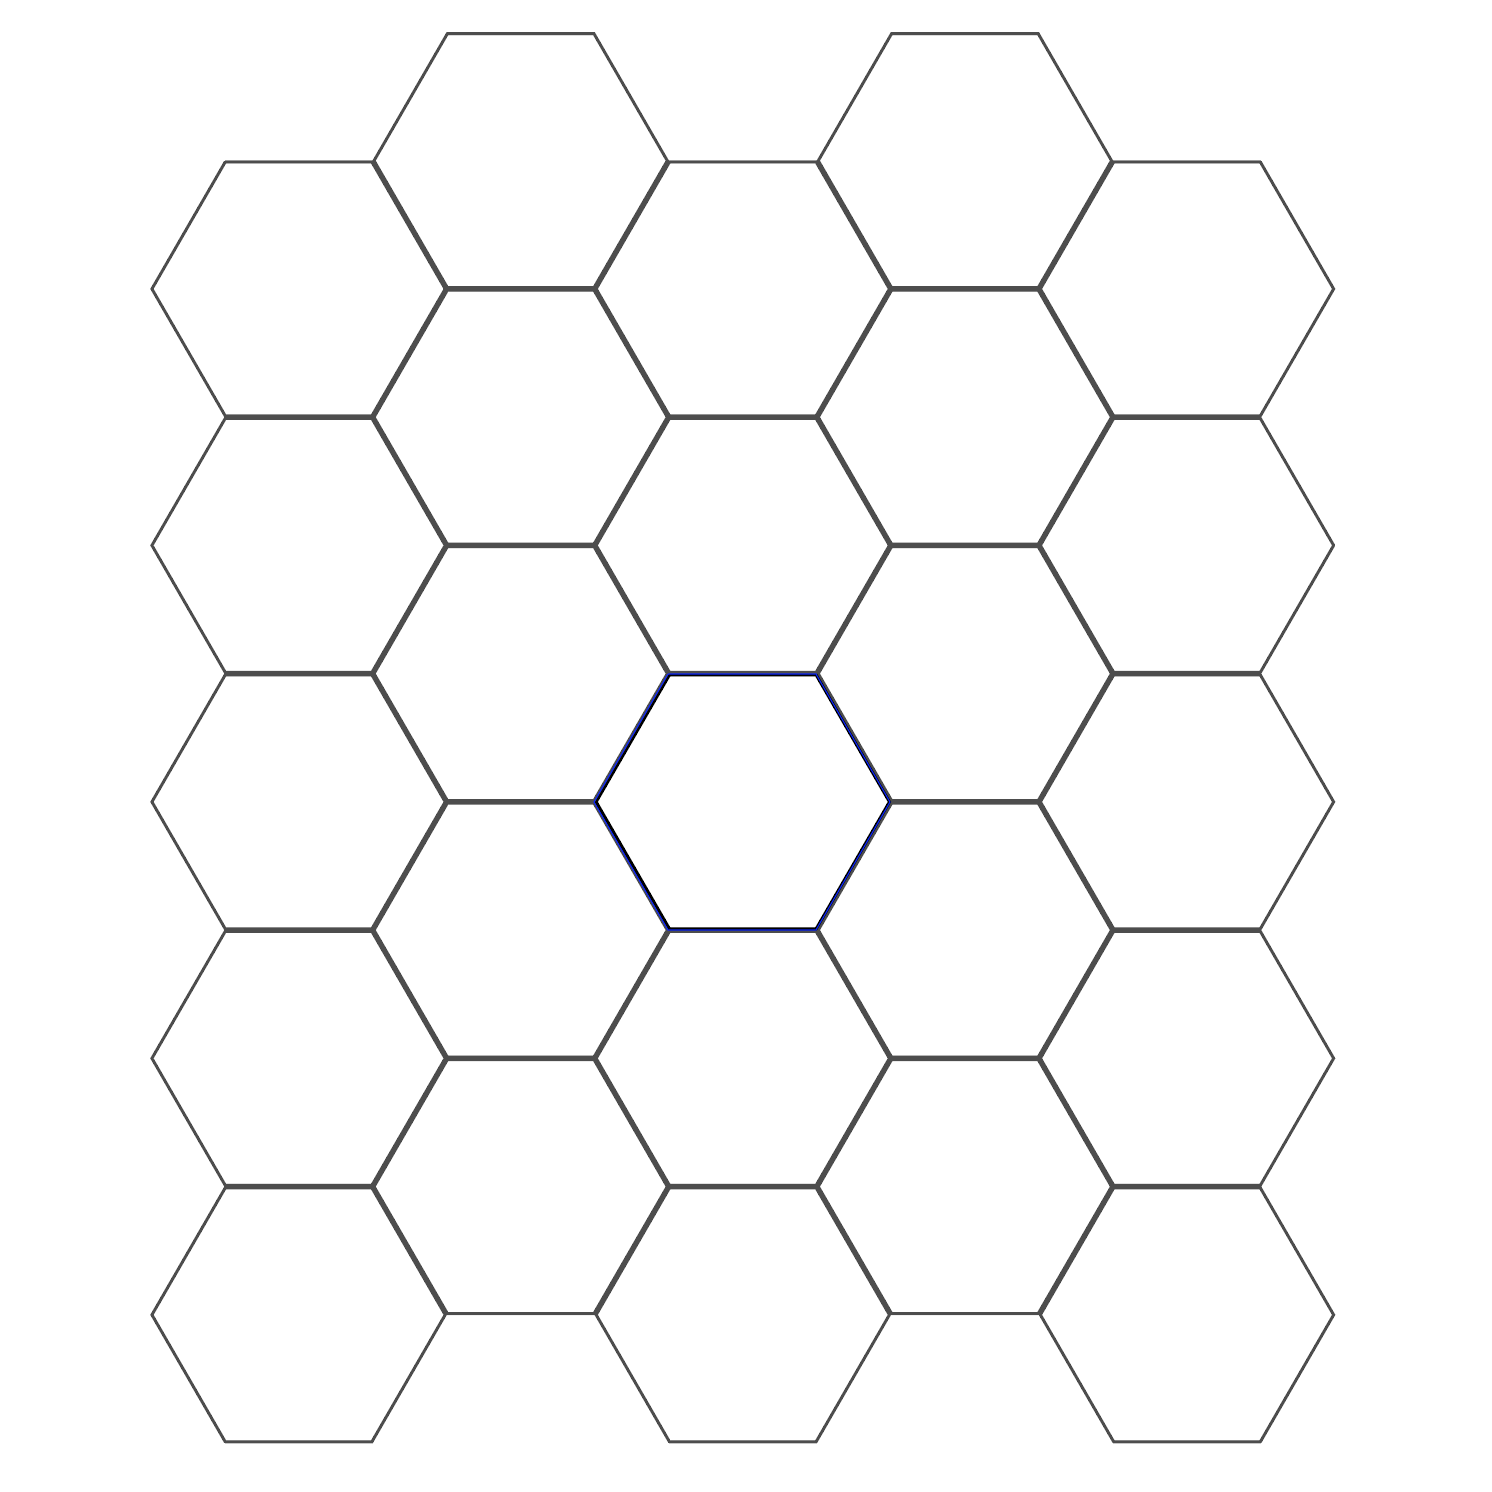
\includegraphics[width=\linewidth]{tes-hex}
            \caption{5x5 tessellation}
        \end{subfigure}
    \end{center}
\end{figure}

\begin{figure}[H]
    \begin{center}
        \caption{Tesselation of a triangle $\{3,6\}$}
        \label{fig:hex}
        \begin{subfigure}[b]{.3\linewidth}
            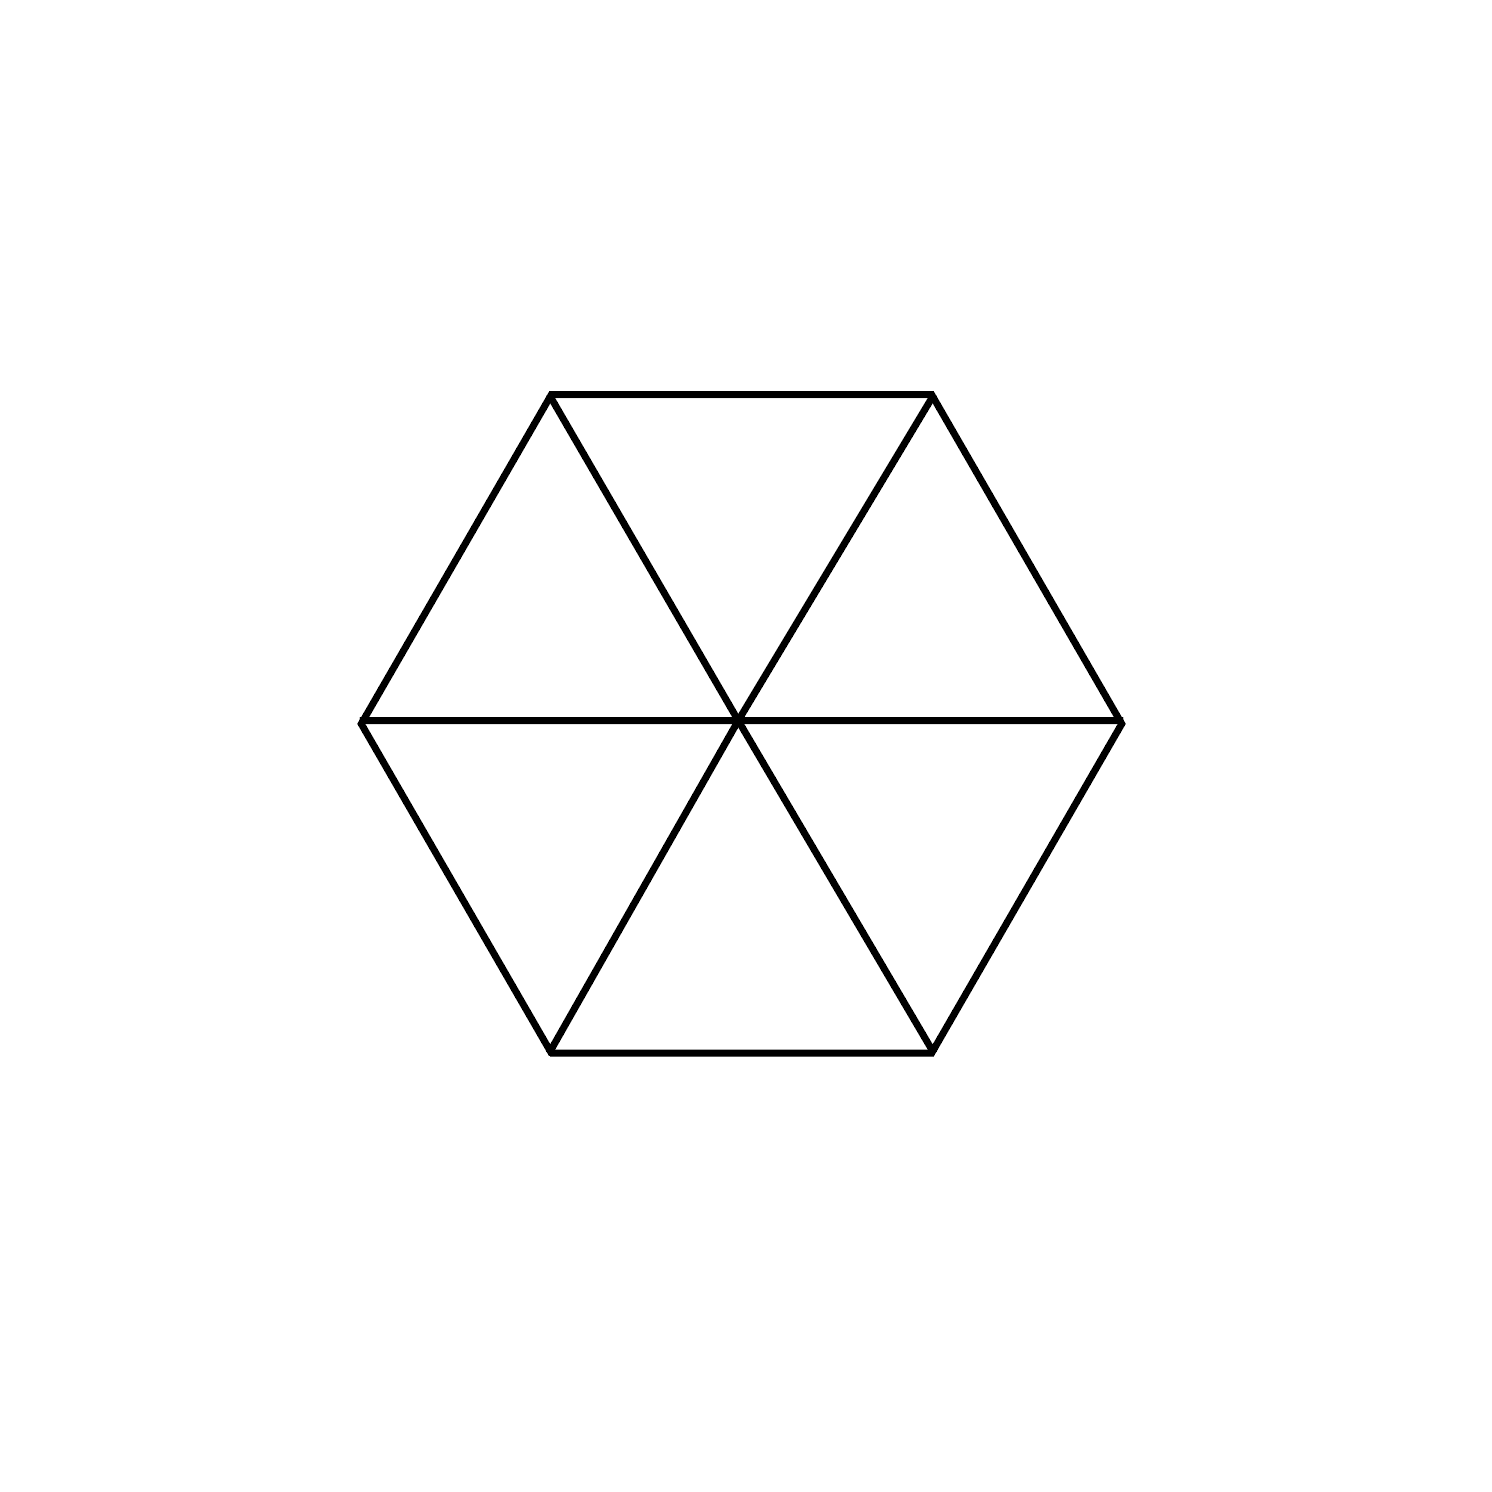
\includegraphics[width=\linewidth]{base-tri}
            \caption{Base 3-sided shape (fits within the base hexagon)}
        \end{subfigure}
        \begin{subfigure}[b]{.3\linewidth}
            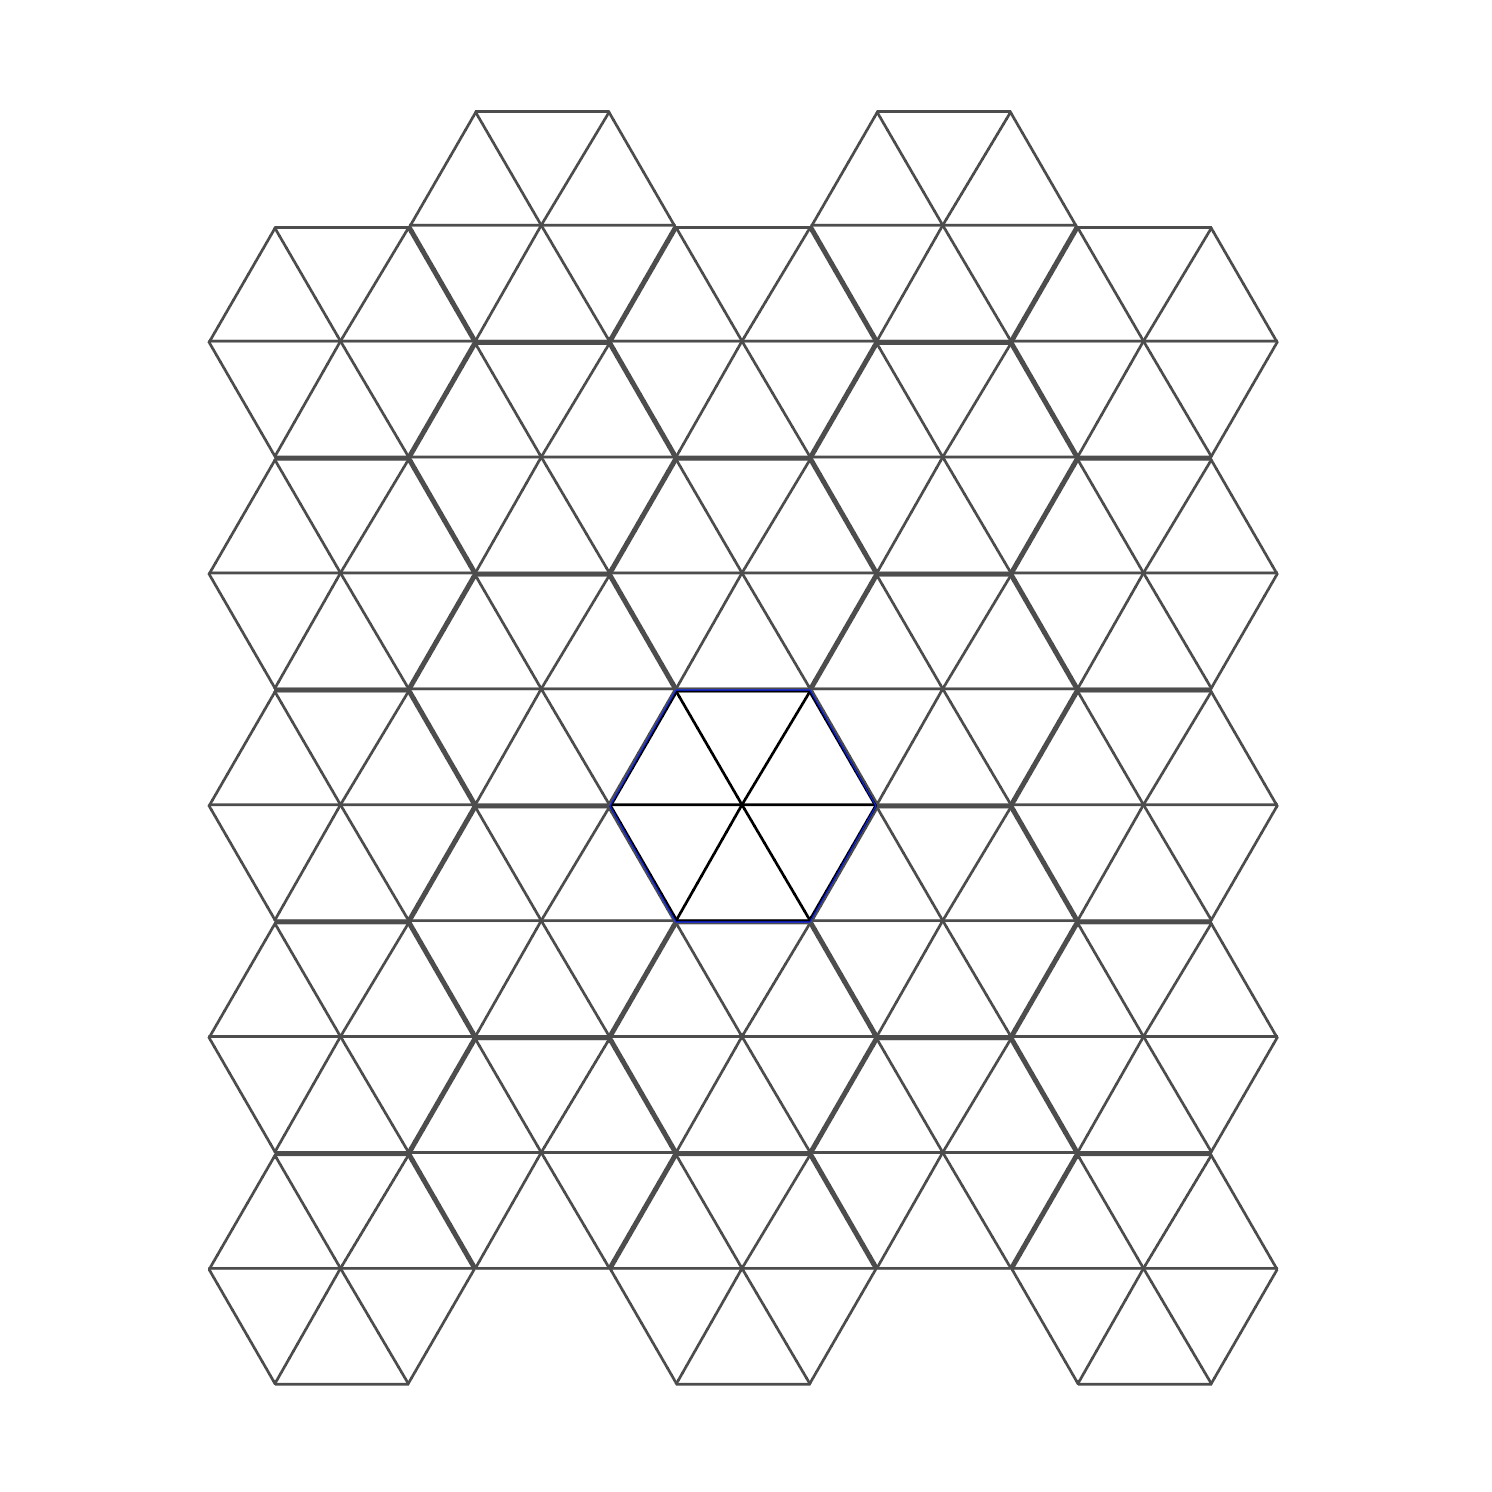
\includegraphics[width=\linewidth]{tes-tri}
            \caption{15x10 tessellation}
        \end{subfigure}
    \end{center}
\end{figure}

It should be noted that many artistic patterns are simply a form of regular tessellation with additional lines and elements within the base shape. For instance, all of the examples of Islamic tessellations in Figure \ref{fig:islam} are abstractions of the regular tessellation $\{6,3\}$.

\section{Practical Applications}
\subsection{Art}
Modern art has adopted tessellation as a common element in futuristic and technical looking designs.
\subsection{Mechanical Engineering}
Tessellation offers a suitable solution for reducing the weight of material without impacting the structural elements of the part. This property of tessellation is why it it frequently used as a hole pattern to make sheet metal parts lighter in the application of robotics. Quadrilateral parallelograms, triangular and hexagonal patterns are the most common in lightening patterns.

\begin{figure}[H]
    \begin{center}
        \caption{Sheet metal plate with a $\{4,4\}$ tessellation pattern}
        \label{fig:belly}
        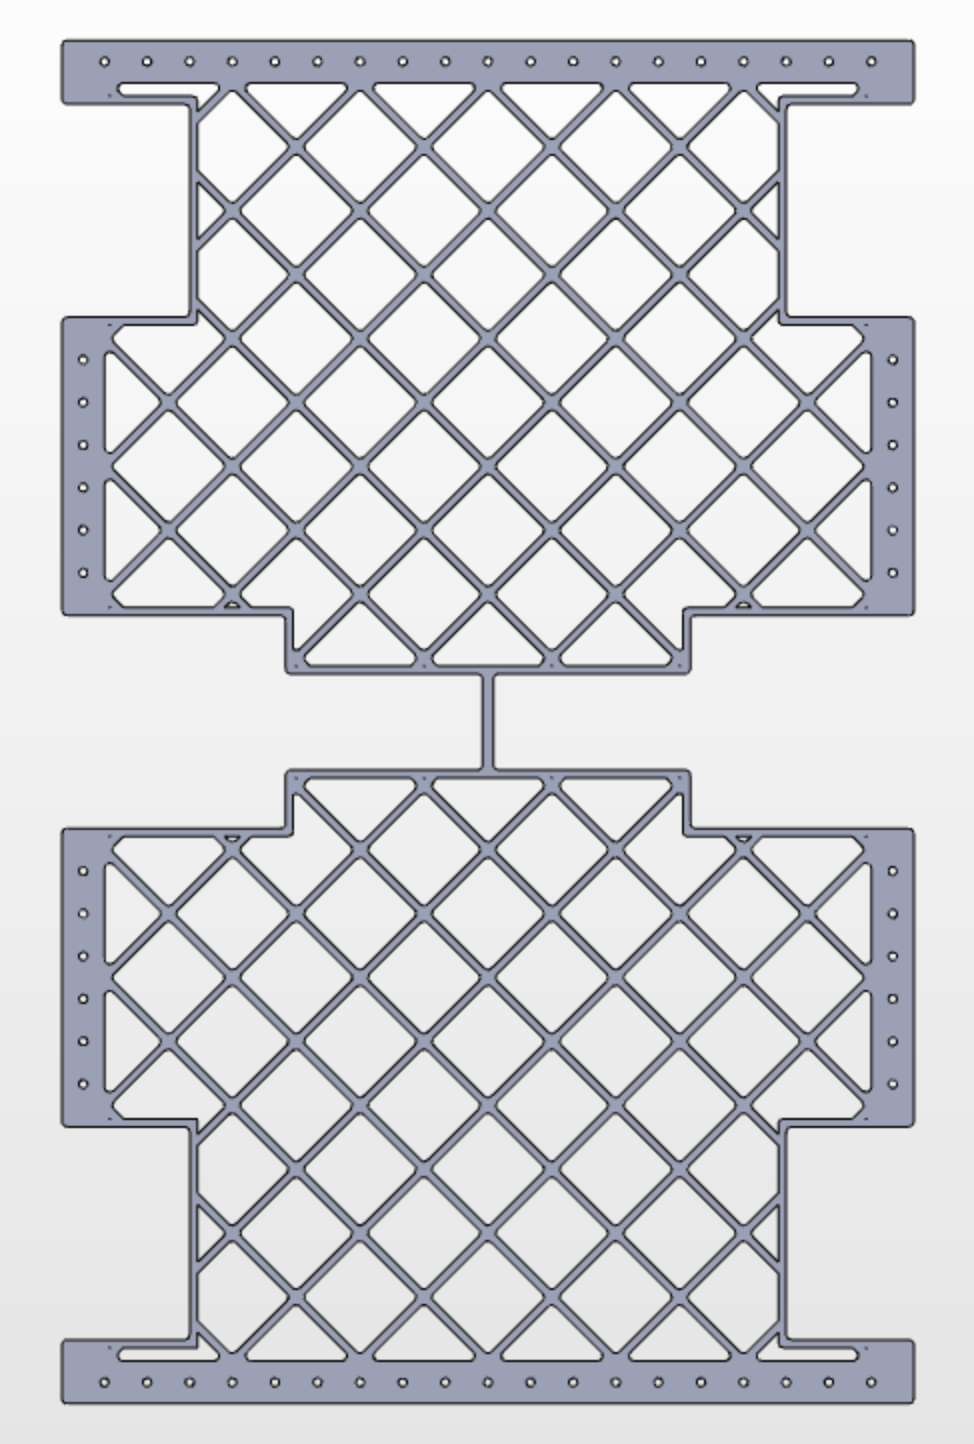
\includegraphics[width=.4\linewidth]{belly}
    \end{center}
\end{figure}

The part shown in Figure \ref{fig:belly} can still distribute compression and tension forces. The application of tessellation patterns in sheet metal part design is one of the main benefits of the material.

\section{Reflection}
\newpage
\bibliography{tynan-math-ia}
\bibliographystyle{apa}
\newpage
\section{Appendix}
\listoffigures
\end{document}